%% 1. 和文「論文」(「解説」を含む)
%% 2. 和文「研究開発レター」
%% 3. 英文「論文/研究開発レター」
%% 4. 英文「Extended Summary」
%%   の各タイプ別のテンプレートです

%% 1. 和文「論文」用テンプレート
\documentclass{ieej}
\usepackage{amsmath,amssymb,epsfig}
\usepackage{graphicx,color}
\usepackage{ascmac}
\usepackage{algorithm,algorithmic}

\def\R{{\Bbb R}}

\def\vec#1{\mbox{\boldmath$#1$}}
\def\sgn#1{\mbox{sgn($#1$)}}
\def\d#1{\mbox{d}}

\def\argmin#1{\underset{#1}{\mbox{argmin~}}}
\def\argmax#1{\underset{#1}{\mbox{argmax~}}}

\renewcommand{\floatpagefraction}{1}
\renewcommand{\topfraction}{1}
\renewcommand{\bottomfraction}{1}
\renewcommand{\textfraction}{0}

\FIELD{C}
\YEAR{2014}
\NO{1}
\jtitle{超関数とカルマンフィルタによる高速な周波数推定}
%\jtitle[]{}
\etitle{Rapid Frequency Estimation of Vital Signs}
\makeatletter
\if@english
\makeatother
\authorlist{%
 \authorentry{Takeshi Nishida}{m}{kit}
 \authorentry{Masuhiro Nitta}{m}{kit}
 }
 \affiliate[kit]{Faculty of Engineering, Kyuchu Institute of
 Technology\\1--1 Sensui, Tobata, Kitakyushu, Fukuoka 804-8550 }{ \\ }
\else
\authorlist{%
 \authorentry{新田 益大}{Masuhiro Nitta}{m}{KIT}
 \authorentry{西田 健}{Takeshi Nishida}{m}{KIT}
% \authorentry{}{}{}{}
}
 \affiliate[KIT]
 {九州工業大学 \\〒804--8550\hskip1zw 福岡県北九州市 戸畑区仙水町 1--1} 
 {Kyushu Institute of Technology \\1--1 Sensui, Tobata, Kitakyushu, Fukuoka 804--8550}
 \affiliate[OEH]
 {産業医科大学産業生態科学研究所 \\〒807--8555\hskip1zw 福岡県北九州市八幡西区医生ヶ丘 1--1} 
 {Department of Ergonomics, Institute of Industrial Ecological Science, 
 University of Occupational and Environmental Health\\1--1 Iseigaoka, Yahata-nishi, Kitakyushu, Fukuoka 807--8555}
%\received{}{}{}
%\revised{}{}{}

\begin{document}
\begin{abstract}
 %
 We propose a novel rapid and highly precise frequency estimation
 method of vital signs.
 %
 The proposed method bases on a notion of distribution theory, and  
 is mathematically stable.  
 %
 The proposed method has adaptation ability and shortens the estimation
 time of the conventional method, such as FFT, dramatically. 
 %
\end{abstract}
\begin{jkeyword}
 超関数推定,
\end{jkeyword}
\begin{ekeyword}
 supper function estimation
\end{ekeyword}
\maketitle

\section{はじめに}
%
医療分野では呼吸数や心拍数などの生体信号の周波数計測は診療の基礎であり,
これを自動計測の手法も数多い.
%
それらの周波数解析には,振動現象の周波数解析技術が用いられ,ノイズ低減を
始めとする高速かつ高精度の振動周波数の推定のための手法は数多く提案されて
いる.
%
一般に広く利用される技術としては高速フーリエ変換(FFT: fast Fourier
transform)による信号のスペクトル密度のピーク探索である.
%
これは,一定時間信号を累積するための窓関数を準備し,その区間の信号におけ
る最も支配的な周波数を探索する手法である.
%
一般に生体信号の周波数は低いため,数秒から数十秒の幅の窓関数を用意する必
要があり,それに伴って,周波数解析結果が算出されるまでの計測時間も長くなる.
%
例えばヒトの呼吸数計測には,一般に5秒から10秒の計測遅れが発生する.


一方,近年,超関数を利用する高速かつ高精度の周波数推定手法が提案されてい
る\cite{SF}.
%
本手法による周波数推定は,20から30のサンプリングデータで高精度の周波数推
定に達成されることが報告されており\cite{SF},振動現象を発生する電子回路
において,その有効性が実証されている.
%
本手法の生態信号解析への応用は未だ実施されていないが,従来手法よりも大幅
な計測時間の短縮を見込める.
%
そこで本研究では,超関数に基づく周波数推定手法を生態信号解析に応用するこ
とを試みる.


\section{超関数による周波数推定の概要}
\subsection{定式化}
次のような単周期信号を考える.
\begin{align}
 x(t)=X_0\cos (\omega t- \theta)
\label{eq:a}
\end{align}
ここで,$X_0$は振幅,$\omega$は各周波数,$\theta$は位相の遅れ角であると
する.
%
まず,この信号の2階の微分方程式は以下のように表せる.
\begin{align}
 \ddot{x}(t)+\omega^2x(t)=0
\label{eq:b}
\end{align}
この関係より,周波数は次のように表現できる.
\begin{align}
 \omega^2=\ddot{x}(t)/x(t)
\label{eq:c}
\end{align}
しかし,離散計測値から$\ddot{x}(t)$を高精度に求めることは一般に困難であ
るため,この関係を実応用に利用することはできない.さらに,微分を利用せず
積分の関係,
\begin{align}
x(t)-x(0)-\dot{x}(0)t+\omega^2\int^t_0\int^{t'}_0x(t'') \mbox{d}t''\mbox{d}t'=0
\label{eq:d}
\end{align}
を利用しても,初期値$x(0)$と$\dot{x}(0)$を高精度に計測することは困難であ
る.

\subsection{超関数の導入}

次の線形関数を考える.
\begin{align}
 \int_{-\infty}^{\infty}f(t)\phi(t)\mbox{d}t
\end{align}
$f(t)$は超関数,$\phi(t)$はテスト関数と呼ばれる.
テスト関数は$C^{\infty}$級関数であり,かつ台がコンパクト,すなわち
\begin{align}
 \lim_{t\to \pm \infty}\frac{\mbox{d}^n\phi(t)}{\mbox{d}t^n} = 0\ \ (n=0,1,2,\cdots)
\end{align}
である.
これらの関数の組み合わせにおいて,次が成り立つ.
\begin{align}
 \int_{-\infty}^{\infty} \frac{\mbox{d} f(t)}{\mbox{d}t}
 \phi(t)\mbox{d}t 
 &=\left[f(t)\phi(t) \right]_{-\infty}^{\infty} -\int_{-\infty}^{\infty} f(t) \frac{\mbox{d} \phi(t)}{\mbox{d}t}
 \mbox{d}t\nonumber\\
 &=-\int_{-\infty}^{\infty} f(t) \frac{\mbox{d} \phi(t)}{\mbox{d}t} \mbox{d}t
\end{align}
したがって,一般に以下が成り立つ.
\begin{align}
 \int_{-\infty}^{\infty} \frac{\mbox{d}^n f(t)}{\mbox{d}t^n}
 \phi(t)\mbox{d}t
 = (-1)^n  \int_{-\infty}^{\infty} f(t) \frac{\mbox{d}^n \phi(t)}{\mbox{d}t^n}
 \mbox{d}t
\end{align}
この関係は,$f(t)$の導関数を$\phi(t)$の導関数で表現できることを意味する.

ここで再び式(\ref{eq:a})の微分方程式を考える.
両辺に$\phi(t)$を乗じて$(-\infty,\infty)$で積分すると,
\begin{align}
 \int_{-\infty}^{\infty}\ddot{x}(t)\phi (t) \mbox{d}t+
 \omega^2 \int_{-\infty}^{\infty}x(t)\phi (t)\mbox{d}t=0
\end{align}
となる.
これを,上述の超関数の性質に従って以下のように記述し直すと,
\begin{align}
 \int_{-\infty}^{\infty}x(t)\ddot{\phi} (t) \mbox{d}t+
 \omega^2 \int_{-\infty}^{\infty}x(t)\phi (t)\mbox{d}t=0
\end{align}
となり,これより,
\begin{align}
\omega^2=-\frac{
 \int_{-\infty}^{\infty}x(t)\ddot{\phi} (t) \mbox{d}t}{
  \int_{-\infty}^{\infty}x(t)\phi (t)\mbox{d}t}
\label{eq:8}
\end{align}
となる.

上述のテスト関数の条件を満たす関数として,ガウス関数を用いることができる.
すなわち,
\begin{align}
\phi(t)=\frac{1}{\sqrt{2\pi \sigma^2}}\exp \left\{-\frac{(t-\mu)^2}{2\sigma^2}\right\}
\end{align}
とし,$\mu$は平均,$\sigma^2$は分散である.
この導関数は以下のようになる.
\begin{align}
\dot{\phi}(t)&=-\frac{t-\mu}{\sigma^2}\phi(t)\\
\ddot{\phi}(t)&=\frac{(t-\mu)^2-\sigma^2}{\sigma^4}\phi(t)
\end{align}

\subsection{推定式の離散化}

次に,式(\ref{eq:8})に関して,有限時間$[T_0, T_0+NT_s]$における積分を考える.
$\mu=NT_s/2$とおき,十分に小さな正の実数$\epsilon$で抑えることができるよう
な$\sigma^2$を利用して$0< \vert \phi(T_0) \vert=\vert \phi(T_0+NT_s) \vert \ll
\epsilon$と仮定すると,次のように近似できる.
\begin{align}
 \int^{\infty}_{-\infty}x(t)\phi(t)\mbox{d}t \simeq 
 \int^{T_0+2\mu}_{T_0}x(t)\phi(t)\mbox{d}t 
\end{align}
さらに区分求積法により,以下のように近似できる.
\begin{align}
 \int^{T_0+2\mu}_{T_0}  x(t)\phi(t)\mbox{d}t  \simeq
 \sum^{N}_{k=0} x(T_0+kT_s)\phi(T_0+kT_s)T_s
\end{align}

以上の関係を利用すると,式(\ref{eq:8})は次のように表せる.
\begin{align}
\omega^2&=-\frac{\sum^{N}_{k=0} x(T_0+kT_s)\ddot{\phi}(T_0+kT_s)}{\sum^{N}_{k=0} x(T_0+kT_s)\phi(T_0+kT_s)}
\end{align}
ここで,$T_0$は任意の計測開始時刻を表す.
一方,式(\ref{eq:a})の$\theta$,すなわち信号の位相ずれに本手法は不変
であるため,次の関係式が成り立つ.
\begin{align}
 \phi(T_0+kT_s)&=\phi(kT_s)\\
 \ddot{\phi}(T_0+kT_s)&=\ddot{\phi}(kT_s)
\end{align}
これらより,
\begin{align}
\omega 
&=\sqrt{
 \sigma^2-
 \frac{\mathbf{q}^T\vec{x}(T_0)}
 {\mathbf{p}^T\vec{x}(T_0)}
 }\biggl/\sigma^2
\end{align}
ここで,
\begin{align*}
 \vec{x}(T_0)&\triangleq 
 \left[ 
 \begin{matrix}
  x(T_0) & \cdots & x(T_0+NT_s) 
 \end{matrix}
 \right]^T\\
%
 \mathbf{p}&\triangleq 
 \left[ 
 \begin{matrix}
  \phi(0) & \cdots & \phi(NT_s) 
 \end{matrix}
 \right]^T\\
%
 \mathbf{q}&\triangleq 
 \left[ 
 \begin{matrix}
  \mu^2\phi(0)  & \cdots & (NT_s-\mu)^2\phi(NT_s) 
 \end{matrix}
 \right]^T
\end{align*}
である.
特に,$\vec{x}(T_0)$の要素が全て充填されるまでの時間$[0,NT_s]$は,$\omega$
の推定は実行されないことに注意が必要である.
また,時刻$NT_s$以降はFIFO形式で$\vec{x}(T_0)$の要素をシフトしながら更
新する.
%
さらに,先行研究における解析から,$N$および$\sigma$,$T_s$
は次の関係を満たす必要があることがわかっている.
\begin{align}
 20T_s <16\sigma < NT_s
\end{align}
多くの事例では$T_s$は計測機器に依存して変更できないため,$N$を定めた後に,
上述の関係を満たす範囲で$\sigma$を定めれば良い.
すると,$\mathbf{p}$と$\mathbf{q}$は計測と無関係であるため,上述のパ
ラメータがが決定されれば計測開始前に一意に設定される.
%
また,計算安定性を確保するために,以下の場合には推定ができない,もしくは
不正確になることに注意する必要がある.
\begin{align}
 \sigma^2-\frac{\mathbf{q}^T\vec{x}(T_0)}{\mathbf{p}^T\vec{x}(T_0)} &<0\\
 \mathbf{p}^T\vec{x}(T_0)&<\varepsilon \ \ (\mbox{e.g.}\  \varepsilon=10^{-6})
\end{align}
これらの場合には,前時刻の推定を継続して利用するとよい.

本手法は,式(\ref{eq:a})に示した振動現象の$X_0$周波数$\omega$の変動をト
ラッキング可能な適応オンライン推定が可能である.
%
ヒトの呼吸数をこの関係で表す場合には,$X_0$および$\omega$,$\theta$は時
変関数で表す必要があるが,定式化においては時不変の定数として扱い,後にこ
れらの変動に適応する機構を考慮する.

\section{シミュレーション}
ここでは,上述の推定手法の性能をシミュレーションにより検証するために,
推定対象として次の信号を用いた.
\begin{align}
 y=\sin(0.5\pi kT_s)
\end{align}
ここで$T_s=0.01$ [s]および$\sigma=((N-20)/2+20)T_s/4$とした.
また,$N$を最小限度の$21$と設定した.

まず,これらの条件におけるテスト関数$\phi(k)$とその2階微分
$\ddot{\phi}(k)$の概形を図\ref{fig:ddphi}に示す.
\begin{figure}[btp]
 \begin{center}
  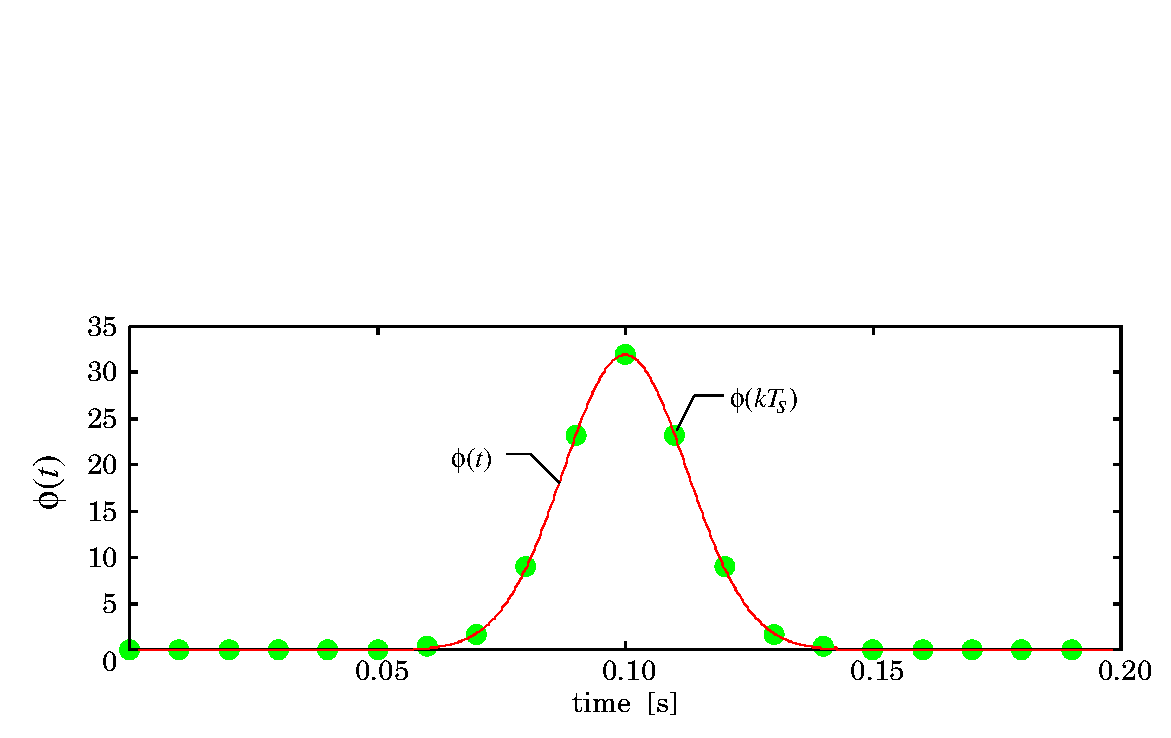
\includegraphics[width=1.0\linewidth]{fig/phi2.eps}\\
  (a) $\phi(k)$\\
  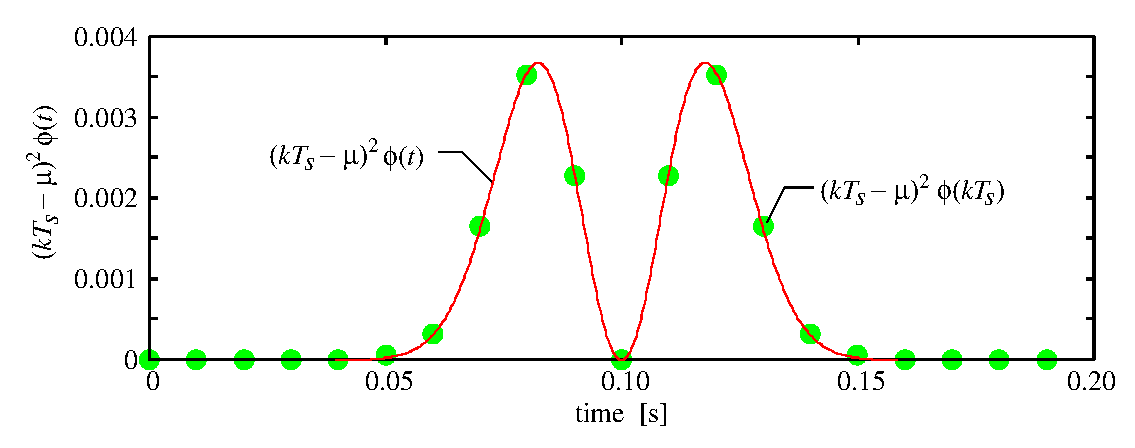
\includegraphics[width=1.0\linewidth]{fig/ddphi2.eps}\\
  (b) $\ddot{\phi}(k)$
 \end{center}
 \caption{The test function of $\mathbf{p}$ and $\mathbf{q}$ ($N=21$).}
 \label{fig:ddphi}
\end{figure}
さらに,それらを利用して推定した結果を図\ref{fig:sim2}に示す.
\begin{figure}[btp]
 \begin{center}
  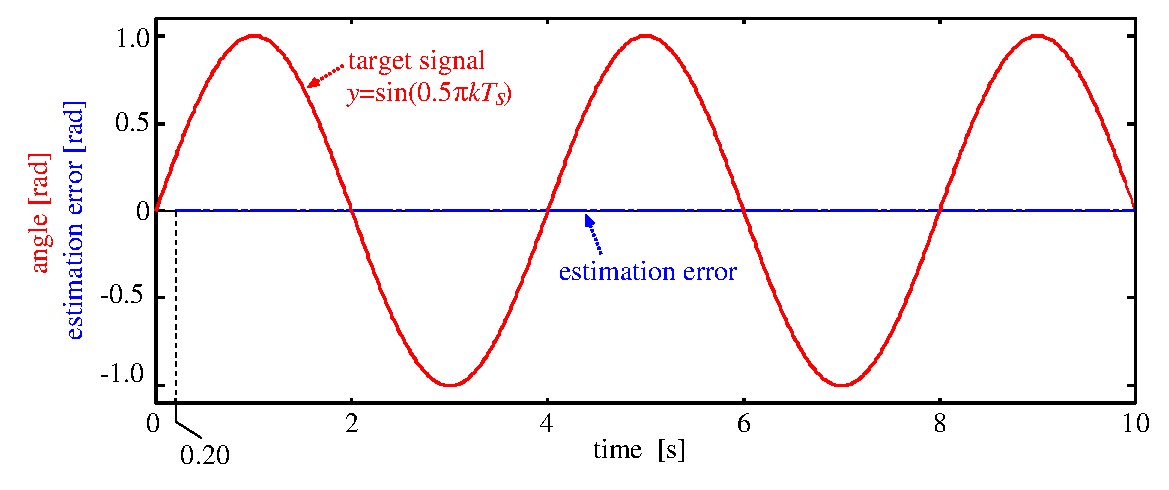
\includegraphics[width=1.0\linewidth]{fig/sim2.eps}
 \end{center}
 \caption{A periodic signal and its frequency estimation results.}
 \label{fig:sim2}
\end{figure}
推定が開始される時刻0.21[s]以降は推定誤差が0であった.
この結果より,単一周期の信号の推定が本手法によって実現されることが示され
た.

\section{実験}


\subsection{呼吸数の推定}

\subsection{心拍数の推定}


\section{おわりに}



\begin{thebibliography}{99}
 \bibitem{SF} A. Ishizaka, M. Nitta, K. Koto, ``Error analysis on
	 distribution-based frequency estimator'', Proc. of
	 Int. Conf. on Control, automation, and Systems, pp. 255--260, 2010.

\end{thebibliography}

\appendix
\section{超関数の性質の導出}

\begin{biography}

\profile{m}{新田 益大}{
平24年より九工大・機械知能工学・助教,博士(工学).
}

\profile{m}{西田 健}{
平10九工大・工・設計生産工卒.
平14九工大大学院博士後期課程修了.同年より九工大・機械知能工学・助手.平
成25年より准教授,博士(工学).屋外移動ロボットに関する研究に従事.日本ロ
ボット学会,計測自動制御学会,日本神経回路学会,電子情報通信学会などの会員.
}

\profile{n}{泉 博之}{
産業医大・産業生態科学研究・人間工学研究室・准教授,博士(工学).
}

%\profile{}{}{}
%\profile*{}{}{}
\end{biography}
\end{document}


%% 2. 和文「研究開発レター」用テンプレート
\documentclass[letter]{ieej}
%\documentclass[mentuke,letter]{ieej}
%\usepackage{graphicx}

\FIELD{}
\YEAR{2014}
\NO{1}
\jtitle{}
%\jtitle[]{}
\etitle{}
\authorlist{%
 \authorentry{}{}{}{}
% \authorentry{}{}{}{}
% \authorentry{}{}{}{}
}
\affiliate[]{ \\ }{ \\ }
%\affiliate[]{ \\ }{ \\ }
%\affiliate[]{ \\ }{ \\ }

%\received{}{}{}
%\revised{}{}{}

\begin{document}
\begin{abstract}

\end{abstract}
\begin{jkeyword}

\end{jkeyword}
\begin{ekeyword}

\end{ekeyword}
\maketitle

\section{}


\begin{thebibliography}{99}% 文献が10以上のとき99,10未満のとき9
\bibitem{}
\bibitem{}
\end{thebibliography}

\appendix
\section{}

\begin{biography}
\profile{}{}{}
%\profile{}{}{}
%\profile*{}{}{}
\end{biography}
\end{document}


%% 3. 英文「論文/研究開発レター」用テンプレート
\documentclass[english]{ieej}
%\documentclass[mentuke,english]{ieej}
%\documentclass[english,letter]{ieej}
%\usepackage{graphicx}

\FIELD{}
\YEAR{2009}
\NO{1}
\title[]{}
\authorlist{%
 \authorentry{}{}{}
% \authorentry{}{}{}
% \authorentry{}{}{}
}
\affiliate[]{ \\ }
%\affiliate[]{ \\ }
%\affiliate[]{ \\ }

%\received{}{}{}
%\revised{}{}{}

\begin{document}
\begin{abstract}

\end{abstract}
\begin{keyword}

\end{keyword}
\maketitle

\section{}


\begin{thebibliography}{99}% 文献が10以上のとき99,10未満のとき9
\bibitem{}
\bibitem{}
\end{thebibliography}

\appendix
\section{}

\begin{biography}
\profile{}{}{}
%\profile{}{}{}
%\profile{}{}{}
\end{biography}
\end{document}


%% 4. 英文「Extended Summary」用テンプレート
\documentclass[english,ExtendedSummary]{ieej}
%\documentclass[english,ExtendedSummary,mentuke]{ieej}
%\usepackage{graphicx}
%\usepackage{latexsym}

\title{}
\authorlist{%
 \authorentry{}{}{}
% \authorentry{}{}{}
}
\affiliate[]{}
%\affiliate[]{}

\begin{document}
\begin{keyword}
% keyword list
\end{keyword}
\maketitle

\end{document}






